\documentclass[11pt]{amsart}
\usepackage[colorlinks=true]{hyperref}
\usepackage{graphicx}
\usepackage{float}
\usepackage{listings}


\title{ScalABM}
\author{David R. Pugh, Daniel F. Tang, J. Doyne Farmer}
\date{\today}

\begin{document}
\maketitle

\section{Objective}
Our objective is to create a \textit{user-friendly} toolkit for building \textit{scalable}, \textit{data-driven} agent-based models (ABMs) of \textit{economic} systems.

\subsection{Requirements}

\subsubsection{...user-friendly...}
We expect that users of our ABM toolkit can be classified as either consumers or producers. Consumers are users whose primary objective is to learn about the mechanisms driving an existing model's key results by playing with model parameters and components. Producers are users whose primary objective is to develop new models using some combination of existing and novel model components.

We want consumers of models built using our framework, particularly those not directly involved with development of any particular model, to be able to easily interact with a model in order to develop intuition and understanding about the mechanisms driving that model's key results.
\begin{itemize}
    \item Models built using our toolkit should have browser-based user interfaces (UIs). Implementing browser-based UIs would allow us to leverage existing, high-quality Javascript libraries for real-time data visualization.
    \item Users should be able to ``play-with'' the model (i.e., tweak model parameters, substitute model components, etc.) from the browser in real-time (i.e., whilst a model is running).
\end{itemize}

We also want to develop a framework that minimizes developer time when either building a new model (or re-configuring an existing model).
\begin{itemize}
    \item Models built using our toolkit should be composed of mostly existing components. This reduces development time for a new model to that needed to create a few novel components together with the time needed to wire all the desired model components together.
    \item The process of wiring model components together, sometimes called dependency injection (DI), should be as simple and transparent as possible.\footnote{
    %
    There are many popular DI approaches (i.e., Guice, Spring, etc). While our framework should not depend on any particular DI library, we should think carefully about what DI library we choose as I expect many users will just mimic our choice.
    %
    }
    \item All model configuration should be done in a \textit{single} file (i.e., some type of application configuration file).  Using this application configuration file it should be possible to reproduce a run of a particular model.
\end{itemize}

\subsubsection{...scalable...}
Aggregate behavior of many (most?) real world social systems fundamentally depends on system size. Therefore in order to accurately model system dynamics we need to be able to run our models as close to observed scale as possible. We need to start thinking about building models ``as if'' we were developing web applications so that we can leverage recent hardware (i.e., massively multi-core servers, cloud computing architectures that are driving the proliferation of large-scale, distributed web applications in private industry.

\subsubsection{...data-driven...}
We want to build models that can be validated against empirical data and therefore we need to design our toolkit to facilitate this.  Again we should think of our models ``as if'' they are web applications. Web applications consume streams of input data and produce streams of output data; some output data streams are processed and then used again as new input data streams. With all of this data flowing around, database integration and data processing are crucial components of web application \textit{design}. We should design our toolkit to integrate cleanly with database architectures, such as \href{http://cassandra.apache.org/}{Apache Cassandra} and \href{http://neo4j.com/}{Neo4j}, and data processing engines, such as \href{http://spark.apache.org/}{Apache Spark}, that are specifically designed to support large-scale web applications.

\subsubsection{...economic...}
Finally, we are not seeking to build a general purpose toolkit for agent-based modeling. Rather we want to build a toolkit that is designed to facilitate the construction of agent-based models of economic systems.

An economy is populated with many seemingly disparate types of agents (i.e., consumers, producers, financiers, government, some markets, etc). We need to distill the core essence (in terms of data and behaviors) of these different agents into a multi-layered Application Programming Interface (API) defining a generic \textit{economic agent} that can then be specialized to the various types of economic agents needed for any particular model. Our hope is that by doing this we can reduce the effort needed for the parts of agent-based modeling that consume a great deal of software development time, such as accounting or contract enforcement.  We also hope that by identifying the key components we can build standard, highly modular interfaces that make it easy to interchange components of models.

\subsubsection{...reproducible...}
Results of many (most?) ABMs are not easily reproducible. More often then not, source code for models used in published articles is not publicly available. Reproducibility is further hindered by the lack of use of ``best practices'' for software development (in particular unit testing). Documentation is typically lacking. 

In order to address these issues and make models built using our toolkit reproducible we should develop the toolkit \textit{from the beginning} as an open-source project and should exemplify ``best practices'' in software engineering: version control using \href{https://git-scm.com/}{Git} and \href{https://github.com/}{GitHub}; continuous integration of unit tests using \href{https://travis-ci.org/}{Travis CI} or \href{https://jenkins-ci.org/}{Jenkins}; static analysis of source code using \href{https://www.codacy.com/login}{Codacy}, \href{https://codeclimate.com/}{Code Climate}, etc; documentation should be extensive, written along with the code, and publicly hosted on GitHub.   
    
\section{High-level design}

\subsection{Platform architecture}
The high-level design of our platform's architecture should mimic the layered architecture of a \href{http://www.reactivemanifesto.org/}{reactive}, ``Fast Data'' web application. Figure \ref{img-figure1} summarizes the high-level design of our platform architecture.\footnote{
%
See figure 1 from \href{./fast-data-big-data-evolved.pdf}{Wampler (2015)} for a similar high-level summary of a Reactive, ``Fast Data'' web application architecture.
%
}
\begin{figure}[H]\label{img-figure1}
\centering
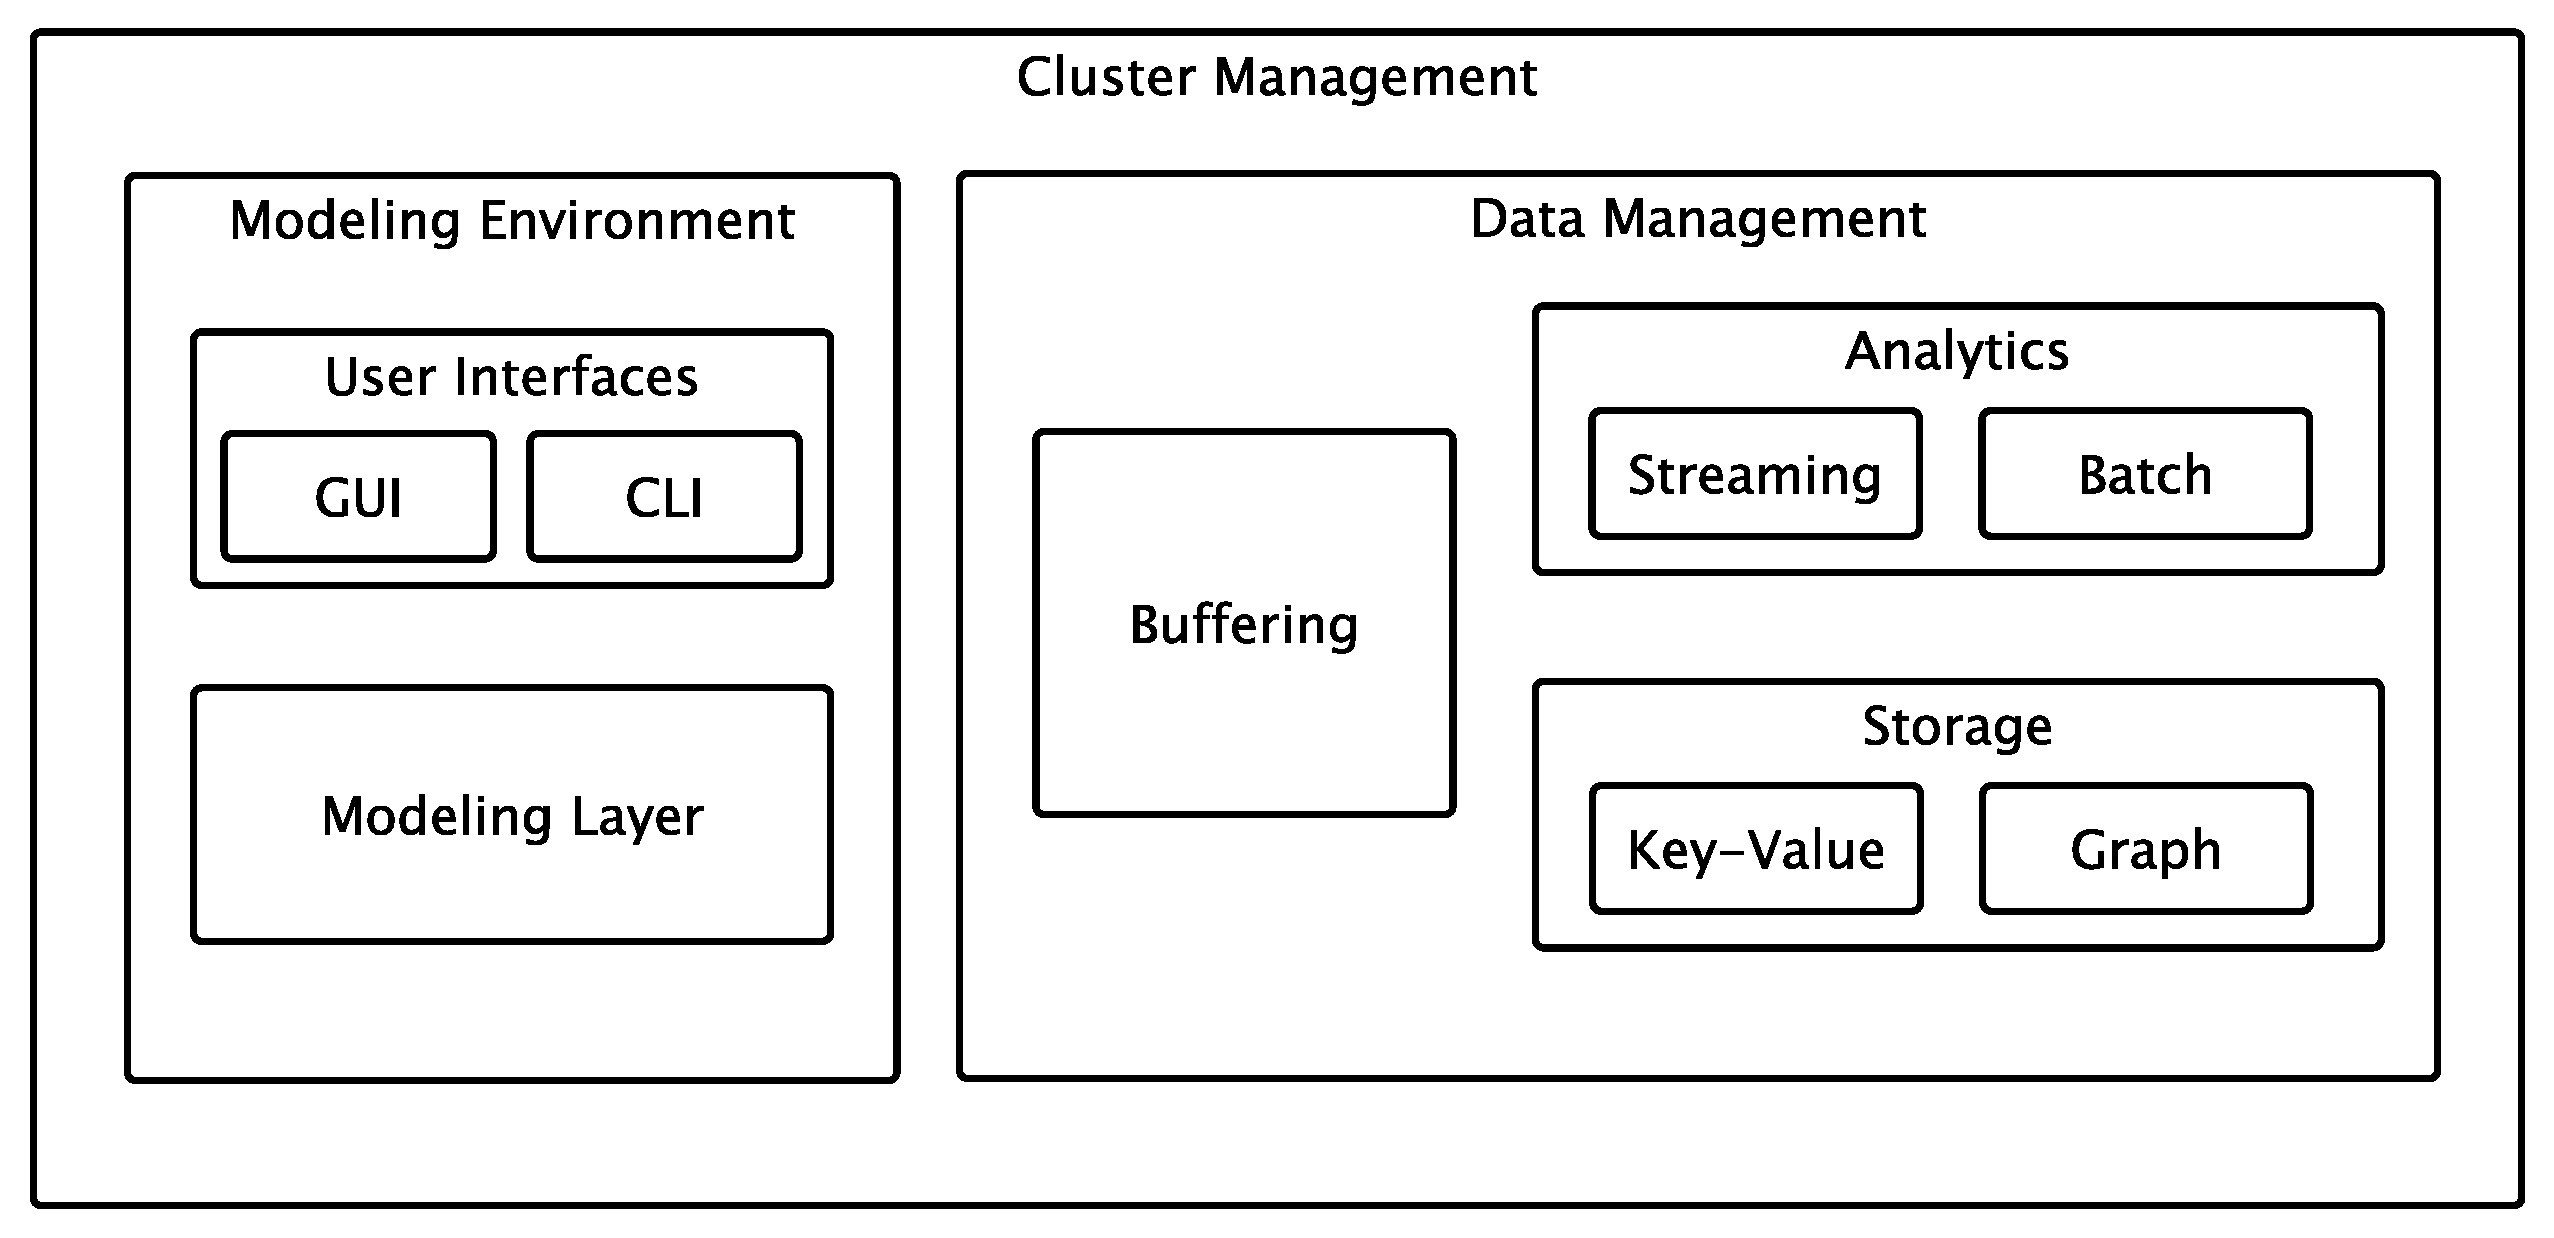
\includegraphics[width=12cm]{img/coarse-grain-schema.pdf}
\caption{High-level architecture design for ScalABM.}
\end{figure}

\subsubsection{Cluster management} 
Current approaches to running large-scale ABMs leverage either...
\begin{itemize}
    \item University/national super-computers: Use FLAME or Repast to build large-scale, complicated models. Both FLAME and Repast use some kind of message passing (but NOT ``peer-to-peer'' message passing) under the hood.
    \item GPU computing: Use CUDA, FLAME GPU (or similar) to build large-scale, simple models.
\end{itemize}
Our strategy for running ABMs at scale will instead leverage massively multi-core cloud computing clusters that are quickly becoming the dominant form of large-scale computing outside of academia.

Benefits to our approach:
\begin{itemize}
    \item Outsourcing of cluster management to third party provider. ABMs built using our framework can be ``containerized'' and sent off to a third-party cloud computing service provider such as \href{http://aws.amazon.com/}{AWS}, \href{https://cloud.google.com/compute/}{Google Compute Engine}, \href{https://www.heroku.com/}{Heroku}, \href{https://mesosphere.com/}{Mesosphere}, etc. This third party provider then handles all of the intricacies involved with scaling up the model on the cluster to meet our needs.
    \item No longer dependent on access to university/national super-computers enhances the reproducibility or our research.  The ability to ``containerize'' an ABM built using out framework means that researchers not directly involved in developing a model can still access all material necessary to completely reproduce that model's output. The container can be used to run the model locally on a laptop or sent to a third party provider to scale up via the cloud. 
\end{itemize}

\subsubsection{Modeling environment}
The modeling environment consists of user interfaces and the modeling layer. The ``front end'' of our modeling environment should consist of two, complementary user interfaces.
\begin{enumerate}
    \item A user-friendly, web-browser based graphical user interface (GUI). The GUI should facilitate interactive exploration of an existing model in near real-time.  The GUI should support real-time data streaming, analysis, and visualization.
    \item An intuitive and consistent command line interface (CLI). In addition to facilitating efficient batch processing of model simulations (i.e., parameter sweeps), the CLI should allow for easy replication of any particular model simulation.
\end{enumerate}

The ``back end'' of our modeling environment is the modeling layer which consists of the actual source code libraries used to implement our ABMs. Important characteristics of our modeling layer:  

\begin{itemize}
    \item The modeling layer should facilitate the construction of new ABMs out of pre-existing, modular components. Novel model components should be able to easily extend pre-existing components. 
    \item Model configuration, including specification of all model parameters as well as the ``wiring'' of model components, should be specified in configuration files that are separate from the actual source code.
\end{itemize}

The modeling layer itself is organized into a number of sub-layers: a behavioral layer, an information layer, and a data analytics layer. See figure \ref{img-figure-2}.
\begin{figure}[H]\label{img-figure-2}
\centering
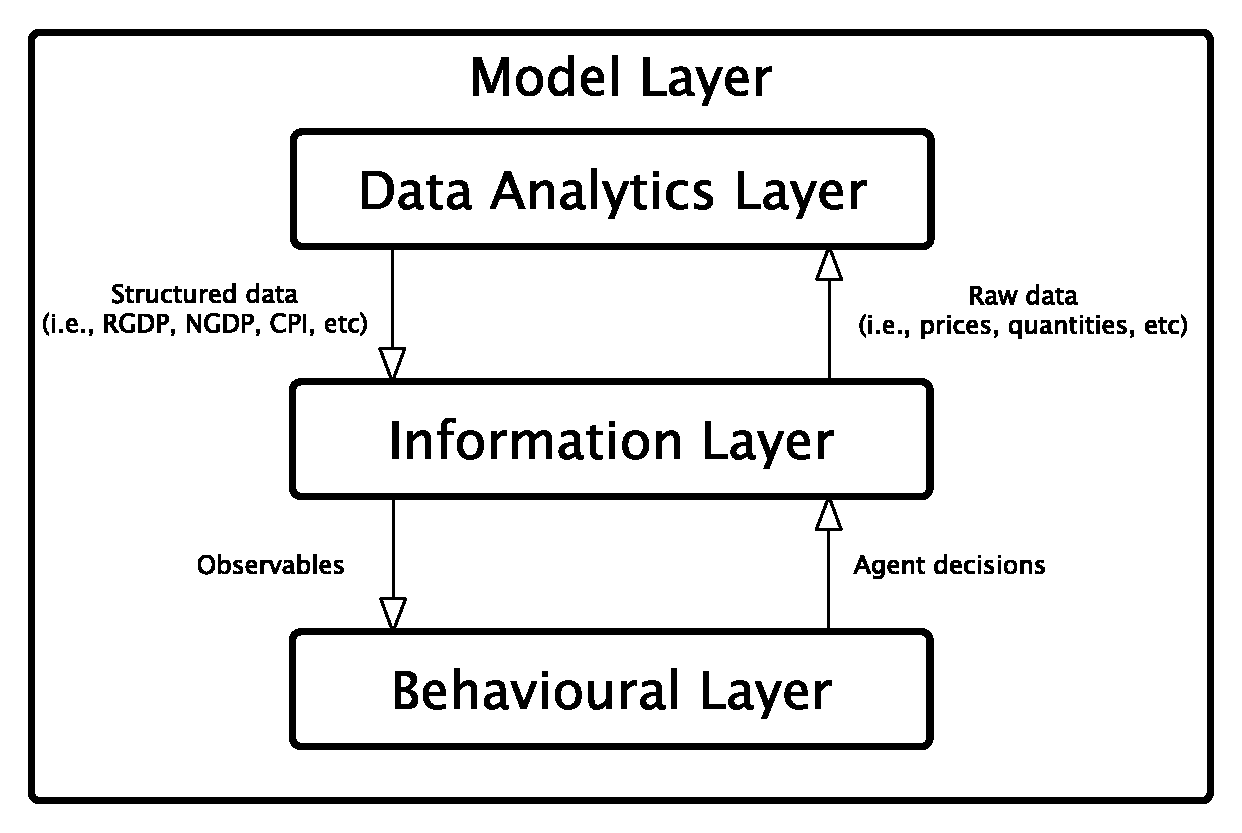
\includegraphics[width=10cm]{img/coarse-grain-model-layer.pdf}
\caption{High-level organization of the modeling layer.}
\end{figure}

\paragraph{Behavioral layer}
An economy is populated with many seemingly disparate types of agents (i.e., consumers, producers, financiers, government, etc).  Our goal with the behavioral layer is to distill the core essence (in terms of data and behaviors) of these different agents into a multi-layered API defining a generic \textit{economic agent} that can then be specialized to the various types of economic agents needed for any particular model.

Several key features distinguish \textit{economic} agents from more generic types of agents. At a minimum these features include: purpose driven (or goal oriented) behaviour, an ability to learn, and the ability to anticipate future events. This suggests that our behavioral layer will need APIs for...
\begin{itemize}
    \item Goals or objectives (and their associated behavioral rules): Our goals/objectives API needs to be as un-opinionated as possible as prospective users of ScalABM are likely to have strong opinions on how to define appropriate goals and decision rules for their agents. At the same time, we will need to have some type of underlying null model of agent goals/objectives. Utility maximization, Belief-Desire-Intent (BDI), probabilistic discrete choice (AKA, random utility maximization) are possibilities.
    \item Learning rules: A large number of various learning rules/mechanisms have been proposed in the academic literature. Roughly, learning rules seem to fall into two camps: learning through previous experience (i.e., reinforcement learning) and learning through observation (i.e., belief learning). Useful references for learning rules for ABMs are the two handbook chapters \href{http://web.uvic.ca/~mingkang/econ353/project/Brenner.pdf}{Brenner (2006)} and \href{http://www.socsci.uci.edu/~duffy/papers/duffy2006.pdf}{Duffy (2006)}.
    \item Expectations formation rules: A large number of various expectation formation rules have been proposed in the literature. Useful references for expectation formation rules are \href{http://feb.kuleuven.be/fac/Slides_Degrauwe/HomHBchapter23.pdf}{Hommes (2006)}, \href{http://econ.columbia.edu/files/econ/content/hommes_background_material_2.pdf}{Anufriev and Hommes (2012)}, \href{http://www.columbia.edu/~mw2230/AREcon.pdf}{Woodford (2013)}, \href{http://www.emeraldinsight.com/doi/pdfplus/10.1108/S0193-230620140000017002}{Assenza et al (2014)}.
\end{itemize}

High-level description of an agent in our framework is a layered collection of behaviors and decision rules...
\begin{figure}[H]
\centering
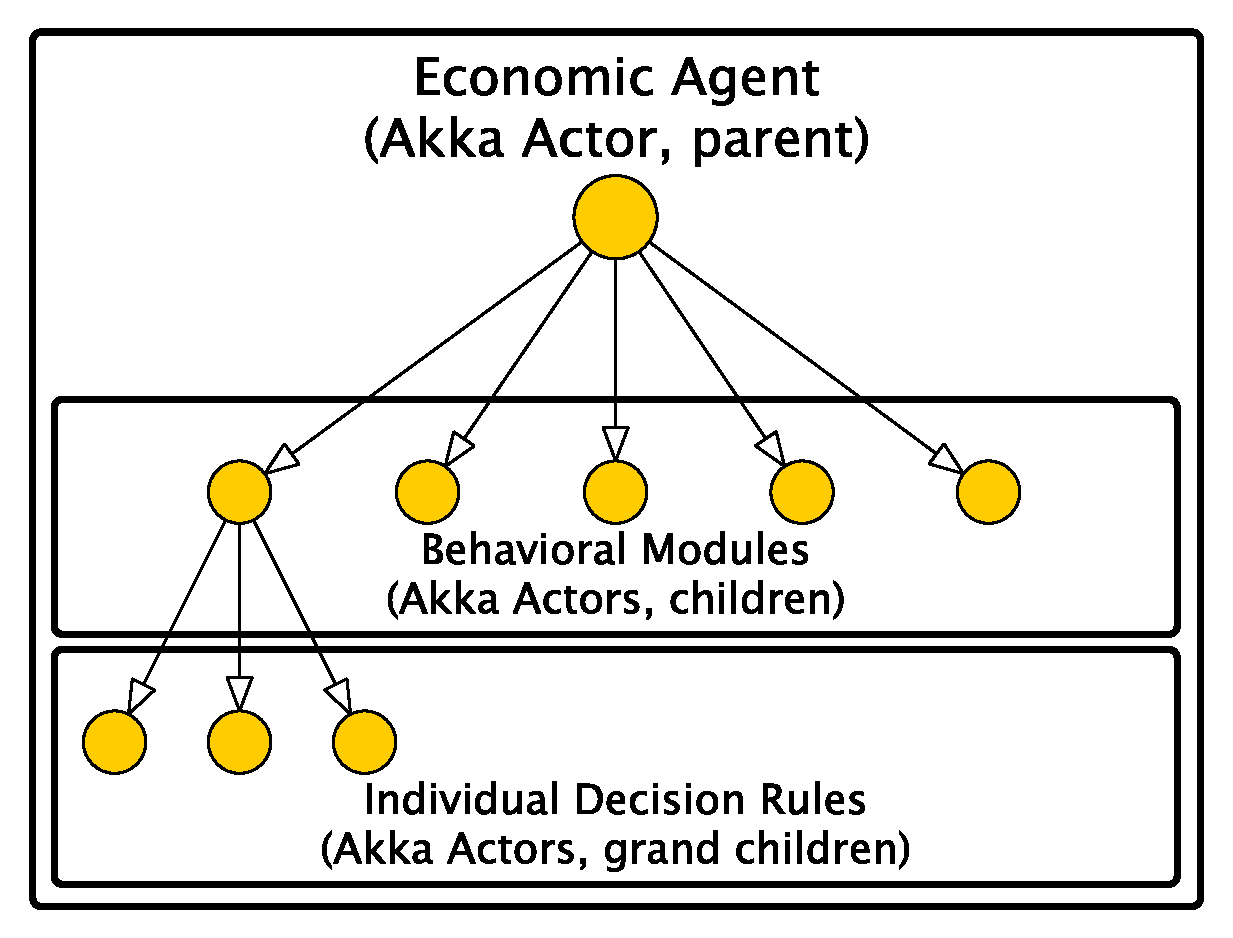
\includegraphics[width=10cm]{img/hierarchical-actor.pdf}
\caption{An agent in our framework is a layered collection of behaviors and decision rules.}
\end{figure}

Concurrent communication between real-world economic agents is a fundamental fact of economic life. Inter-agent communication can be either direct (i.e., ``peer-to-peer'') or indirect (i.e., via market institutions). In order to model both direct and indirect communication between economic agents in our framework we leverage the \href{https://en.wikipedia.org/wiki/Actor_model}{Actor model} of concurrency.   to model both direct and indirect communication between economic agents as concurrent, asynchronous message passing.

t treats ``actors'' as the universal primitives of concurrent computation: in response to a message that it receives, an actor can make local decisions, create more actors, send more messages, and determine how to respond to the next message received.

Stock flow consistency is an important property of large-scale macro models, but is not a property that makes sense to impose in general for our framework.  Need to have a behavioral module that implements stock flow consistent accounting rules.

% \subsection{\texttt{CounterpartyActor} API}
% Perhaps surprisingly, some economists have already been thinking along these lines:

% \begin{quote}
% ``To analyze how financial commitments affect the economy it is necessary to look at economic units in terms of their cash flows. The cash-flow approach looks at all units -- be they households, corporations, state and municipal governments, or even national governments -- as if they were banks.''
% \end{quote}

% The above quotation is taken from Hyman Minsky's magnum opus ``Stabilizing an Unstable Economy.''  Following Minsky,
% and more recently Perry Mehrling, we view every \texttt{EconomicActor} as an entity that is both receiving certain cash flow events (i.e., receipts of various kinds) as well as generating cash flow events (i.e., expenditures of various kinds).\footnote{
% %
% Both Minsky and Mehrling subscribe to the ``banking perspective''. Within the banking perspective, the most basic constraint that all economic actors face is the \textit{survival constraint}: the inflow of receipts must be at least as big as the outflow of expenditures events. Put another way, maintaining sufficient liquidity is the primary concern for all economic actors; solvency (i.e., in the positive net worth sense) is a secondary concern.
% %
% }

% The time pattern of cash flow events for a particular \texttt{EconomicActor} will be primarily determined by the various contractual arrangements to which it is a \textit{counterparty}.  Thus, in our framework, every \texttt{EconomicActor} is also a \texttt{CounterpartyActor}. The accumulation, across time, of cash flow events for a particular \texttt{CounterpartyActor} is captured by its \textit{balance sheet}.

% \subsubsection{Requirements for a \texttt{CounterpartyActor}}
% Quick list of current requirements for a \texttt{CounterpartyActor}:
% \begin{itemize}
%     \item a \texttt{CounterpartyActor} should have a \texttt{BalanceSheet},
%     \item a \texttt{CounterpartyActor} should be able to process cash flow events.
% \end{itemize}

% \subsubsection{Requirements for a \texttt{BalanceSheet}}
% Quick list of current requirements for a \texttt{BalanceSheet}:
% \begin{itemize}
%     \item a \texttt{BalanceSheet} should have a collection of \texttt{ContractActor} objects representing assets, 
%     \item a \texttt{BalanceSheet} should have a collection of \texttt{ContractActor} objects representing liabilities,
%     \item a \texttt{BalanceSheet} should be able to compute its equity.
% \end{itemize}

% \subsubsection{Requirements for a \texttt{ContractActor}}
% Quick list of current requirements for a \texttt{ContractActor}:
% \begin{itemize}
%     \item a \texttt{ContractActor} is a \texttt{CommunicatingActor},
%     \item a \texttt{ContractActor} should have an issuer for whom the \texttt{ContractActor} is a liability, 
%     \item a \texttt{ContractActor} should have a counterparty for whom the \texttt{ContractActor} is an asset,
%     \item a \texttt{ContractActor} should have a \texttt{Commitment} specifying the terms of the agreement between the issuer and the counterparty,
%     \item a \texttt{ContractActor} should be able to value its \texttt{Commitment}.
% \end{itemize}
% Conceptually, a \texttt{ContractActor} represents a channel for communication between the issuer and the counterparty to the underlying \texttt{Commitment}.
Our economic agents will need to condition their decisions on an information set.  In contrast to (most) DSGE models, information sets in our framework will be highly heterogeneous. The information set for any particular economic agent should consist of three components:
\begin{itemize}
    \item Private information: information that is idiosyncratic to a particular agent. 
    \item Public information: information that a particular agent shares with one or more agents.
    \item Global information: information that is shared between all agents.
\end{itemize}

\begin{figure}[H]
\centering
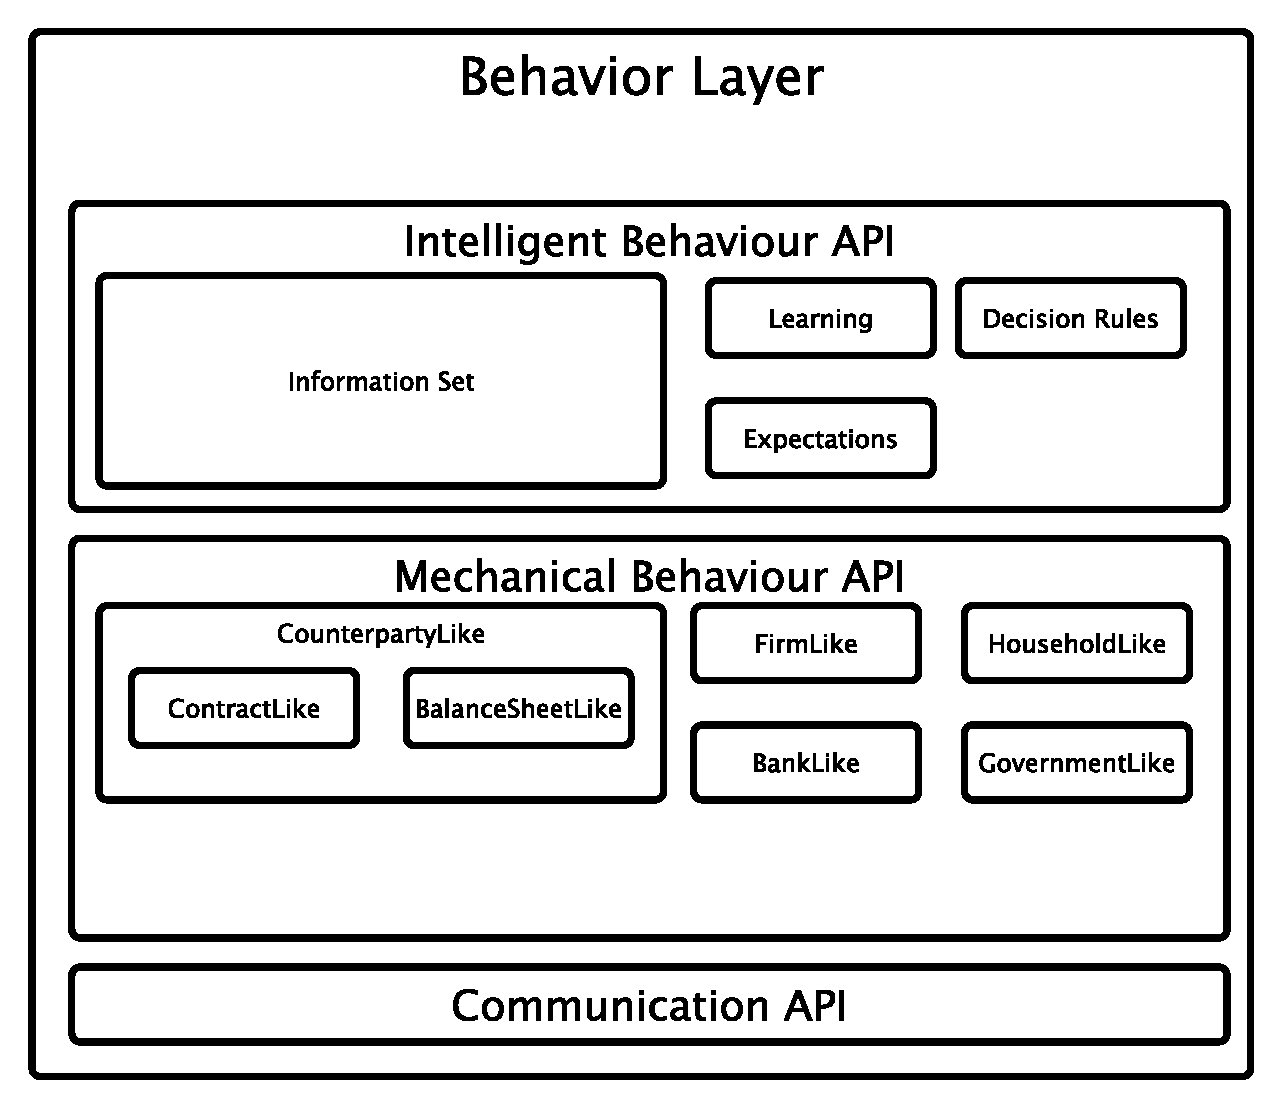
\includegraphics[width=10cm]{img/behavior-layer.pdf}
\caption{???}
\end{figure}


\paragraph{Information Layer}
Markets are institutions that aggregate data: markets take agent decisions/choices as raw data which they aggregate into prices and quantities. These prices and quantities are, typically, but not always observable by others.  Most market prices are public information.
\begin{figure}[H]
\centering
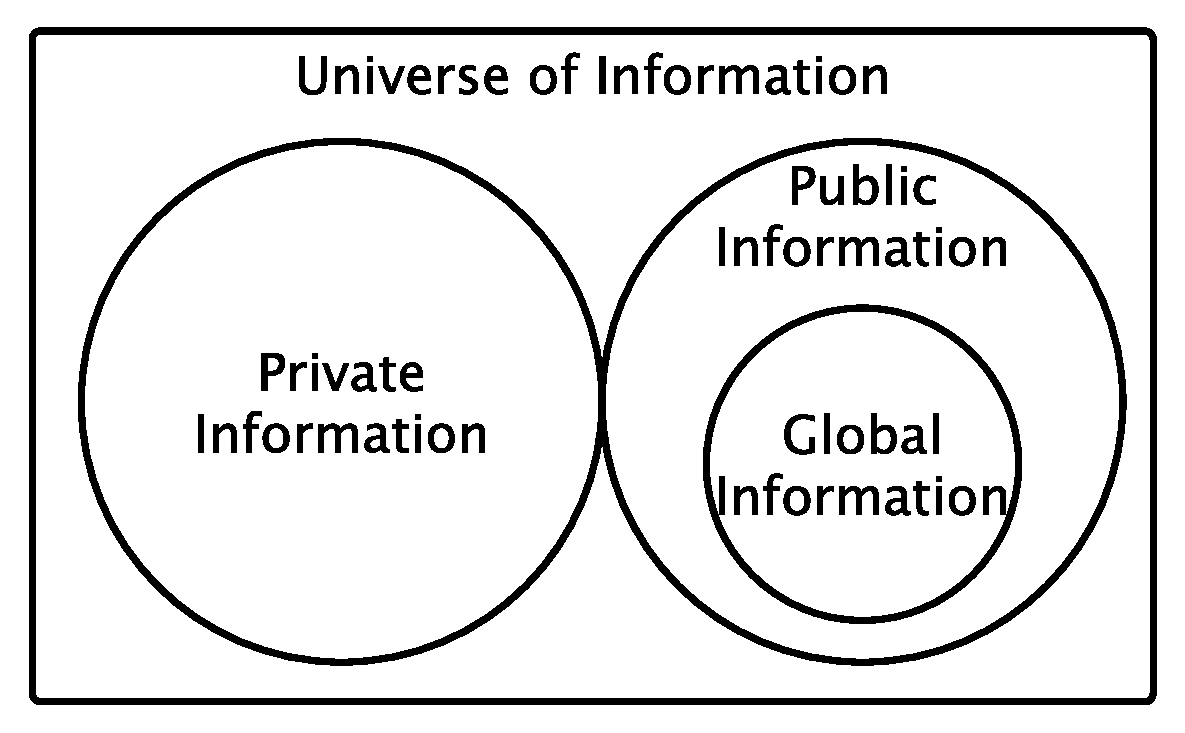
\includegraphics[width=10cm]{img/information-sets.pdf}
\caption{Information set for a particular economic agent.}
\end{figure}

\begin{figure}[H]
\centering
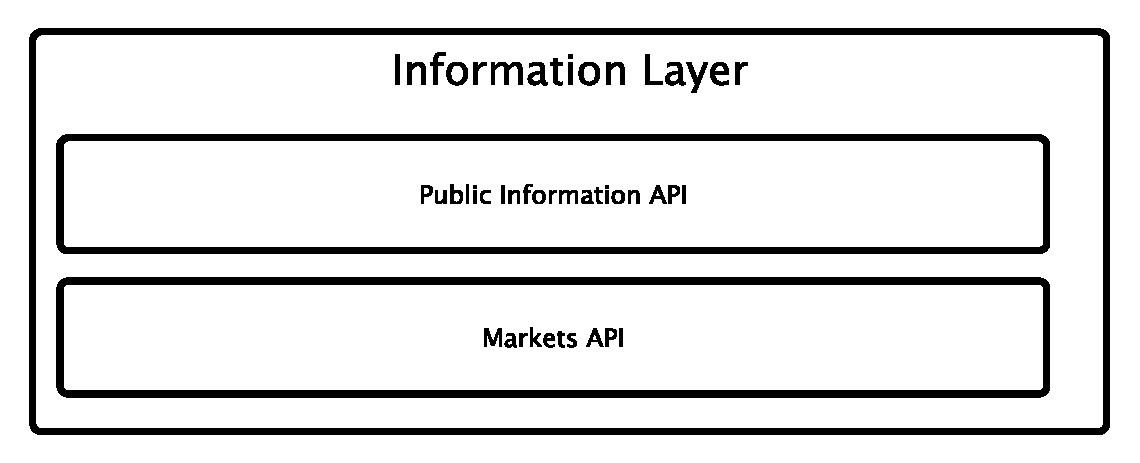
\includegraphics[width=10cm]{img/information-layer.pdf}
\caption{Information layer consists of the markets API and a public information API.}
\end{figure}

\paragraph{Data Analytics Layer}
The data analytics layer encapsulates the functionality for aggregating raw data into additional structured data that agents can use for making decisions.  Specifically, the data analytics layer would contain classes and methods for computing standard macro economic indicators (i.e., real and nominal GDP, stock market index, house price index, consumer price index, unemployment rates, etc). Users should be able to extend the data analytics capabilities as needed for a particular model.


\subsubsection{Data Management}
In order for our ABMs to be data-driven, we need to think carefully about how our framework we will manage the flow and storage of data (both model generated data as well as real-world data). There are (at least!) three components to data management: access, analytics, and storage.
\begin{itemize}
    \item Access: A running ABM will generate a large volume of data. Model generated data might be stored, sent to a data analytics engine, or logged out to a file(s). Additionally, data will likely flow in the reverse direction.  In particular, agents in a running ABM may need to read data from a data store (for example, we might wish to initialize economic agents using real-world data).
    \item Analytics: A running ABM is a continuous source of data whose volume is not predetermined. Put another way: ABMs generate \href{http://www.reactive-streams.org/}{reactive data streams}.  Our data analytics components should therefore include tooling for processing and analyzing streaming data. In addition to processing and analyzing streaming data, we will also need to preform various ``batch'' or ``mini-batch'' computations. Such batch processing jobs would be performed either relatively infrequently on streaming data or upon completion of a model simulation. Our data analytics should include tooling for dealing with batch computations.
    \item Storage: The modeling layer should have read/write access to a scalable data store. Additionally, the data analytics components will need a source of input data. In order to avoid simulations being I/O bound, our data store should have extremely fast write access.
\end{itemize}

\section{Implementation}

\subsection{Platform architecture}

\begin{figure}[H]
\centering
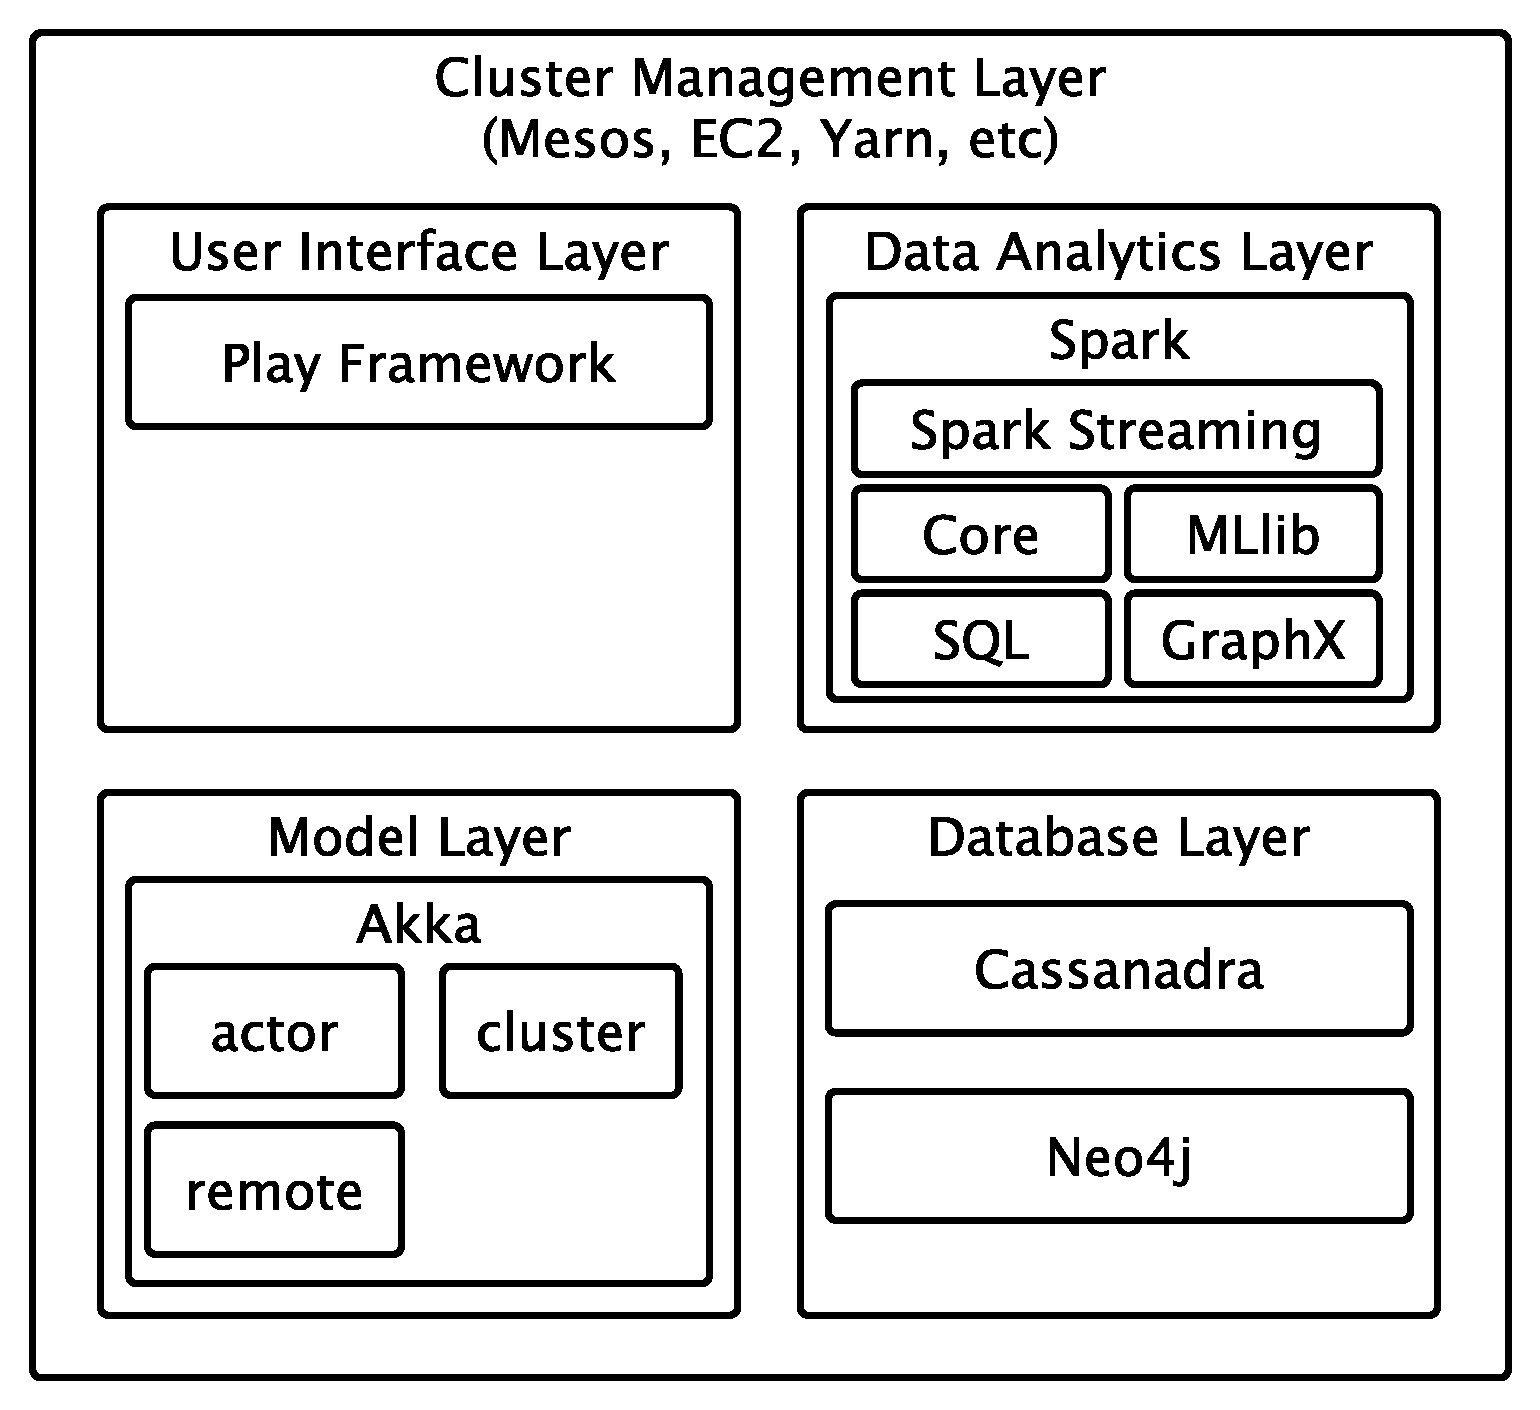
\includegraphics[width=10cm]{img/coarse-grain-schema-2.pdf}
\caption{Macro-grain architecture for ScalABM. }
\end{figure}

\subsubsection{Modeling environment}
Browser based GUI interfaces should be built using the \href{https://www.playframework.com/}{Play} web application framework. The Play framework cleanly integrates Javascript libraries for real-time data analysis and visualization with backend model libraries.

\subsubsection{Data Management}
Broadly speaking, we will need to store two types of data: real-world data and model generated data. The way in which we store our data should be heavily influenced by the types of questions we intend to ask of our data. 
There are two kinds of questions that we will want to ask of our model generated data:
\begin{enumerate}
    \item Questions about cross-sectional and time series properties of model generated data. For these types of questions NoSQL Key-Value databases, such as \href{http://cassandra.apache.org/}{Cassandra},  are ideal data stores. Key-Value databases are designed for storing data in a schema-less way. In a key-value store, each datum consists of an indexed key and a value, hence the name. 
    \item Questions about the network structures between model agents. For questions about network structure, graph databases are ideal.  Graph databases, such as Neo4j, are designed for data whose relations are well represented as a graph and has elements which are interconnected, with an undetermined number of relations between them.
\end{enumerate} 


\subsection{Modeling Layer}
ScalABM leverages the \href{https://en.wikipedia.org/wiki/Actor_model}{Actor model} of concurrency as implemented in the \href{http://akka.io/}{Akka} library to model both direct and indirect communication between economic agents using concurrent, asynchronous message passing.\footnote{
%
Akka is a toolkit and runtime for building highly concurrent, distributed, and resilient message-driven applications on the JVM.
%
}
\begin{figure}[H]
\centering
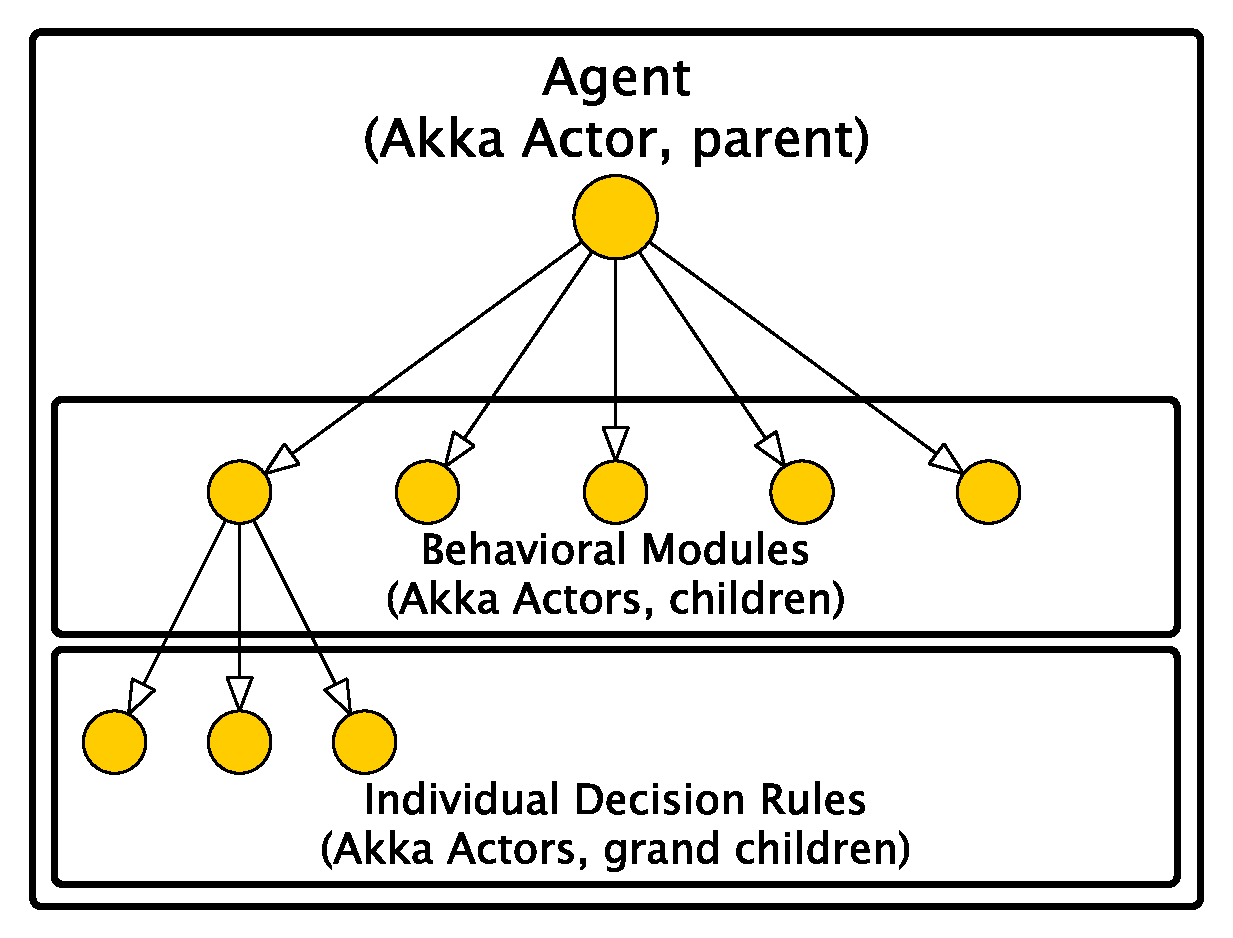
\includegraphics[width=10cm]{img/hierarchical-actor-2.pdf}
\caption{???}
\end{figure}

\subsubsection{Communication Layer}
In order to impose structure on inter-agent communications we have developed an API for a scalable agent communication language for economic agents tentatively called ScalACL. ScalACL leverages the \href{https://en.wikipedia.org/wiki/Actor_model}{Actor model} of concurrency as implemented in the \href{http://akka.io/}{Akka} library to model both direct and indirect communication between economic agents using concurrent, asynchronous message passing.\footnote{
%
Akka is a toolkit and runtime for building highly concurrent, distributed, and resilient message-driven applications on the JVM.
%
}
The ScalACL API specifies...
\begin{itemize}
    \item a set of abstract message types that impose structure on the messages passed between a group of economic agents,
    \item a set of abstract protocols that impose structure on conversations (i.e., sequences of messages) between a group of economic agents,
    \item a behavioral trait that allows an agent to communicate using the language.
\end{itemize}
Each abstract message type can be thought of as defining an ``envelope'' containing the actual content of the message that is to be exchanged between a group of economic agents. Defining envelopes containing messages is useful because it allows agents to react based on the type message received. Each abstract protocol defines a particular subset of message types that can be sent by an agent in response to a particular type of message that it has received. 

Our agent communication API is influenced by, but not slave to, the \href{http://www.fipa.org/}{Foundation for Intelligent Physical Agents (FIPA)} compliant \href{http://www.fipa.org/specs/fipa00037/SC00037J.pdf}{Agent Communication Language (ACL)}.

% \section{Economics as distributed computation}
% Major source of motivation for our approach is Rob Axtell's \href{http://www.researchgate.net/profile/Robert_Axtell2/publication/228586815_Economics_as_distributed_computation/links/0a85e536b81c27f06e000000.pdf}{2002 Brookings working paper}.

% \subsection{Concurrency vs parallelism}
% Discuss the difference between parallelism and concurrency. See this \href{http://stackoverflow.com/questions/1050222/concurrency-vs-parallelism-what-is-the-difference}{SO} post for details. Concurrency is a more general type of parallelism. Economic systems are concurrent.

% \subsection{Asynchronous vs synchronous}
% Discuss the difference between synchronous and asynchronous execution. Economic systems are asynchronous not synchronous.

% \subsection{Economics is concurrent, asynchronous distributed computing}
% Concurrent, asynchronous In his , Rob discusses have noted that the economy is a distributed system which provides a motivation for our use of Scala and Akka to implement our framework (both were developed specifically for building scalable distributed systems). Contrast with other ABM frameworks, programming lanaguages, etc.

%There is a sense in which economics can be reduced to a combination of accounting and agent decision making.  

\end{document}
